\documentclass[xetex,aspectratio=43]{beamer}

\usepackage{res/lections}

\preamble

\title[Современные асинхронные шины]{Современные асинхронные шины}

\begin{document}

\titleslide

\tocslide

\section{Что делать с выравниванием длины дорожек?}

\begin{frame}{А зачем нужны асинхронные последовательные шины}
    \begin{enumerate}
        \item Что нам мешает?
        \begin{enumerate}
            \item Противостояние тактовая частота --- скорость света
            \item «Широкая» шина
        \end{enumerate}
        \pause
        \item На <<узкой>> шине выровнять дорожки легче. До сих пор <<держатся>> параллельными дорожки к ОЗУ, и то с оговорками, но об этом позже
    \end{enumerate}
\end{frame}

\section{Внутренняя шина PCI Express}

\begin{frame}{PCI Express: Root Complex}
	\begin{figure}
        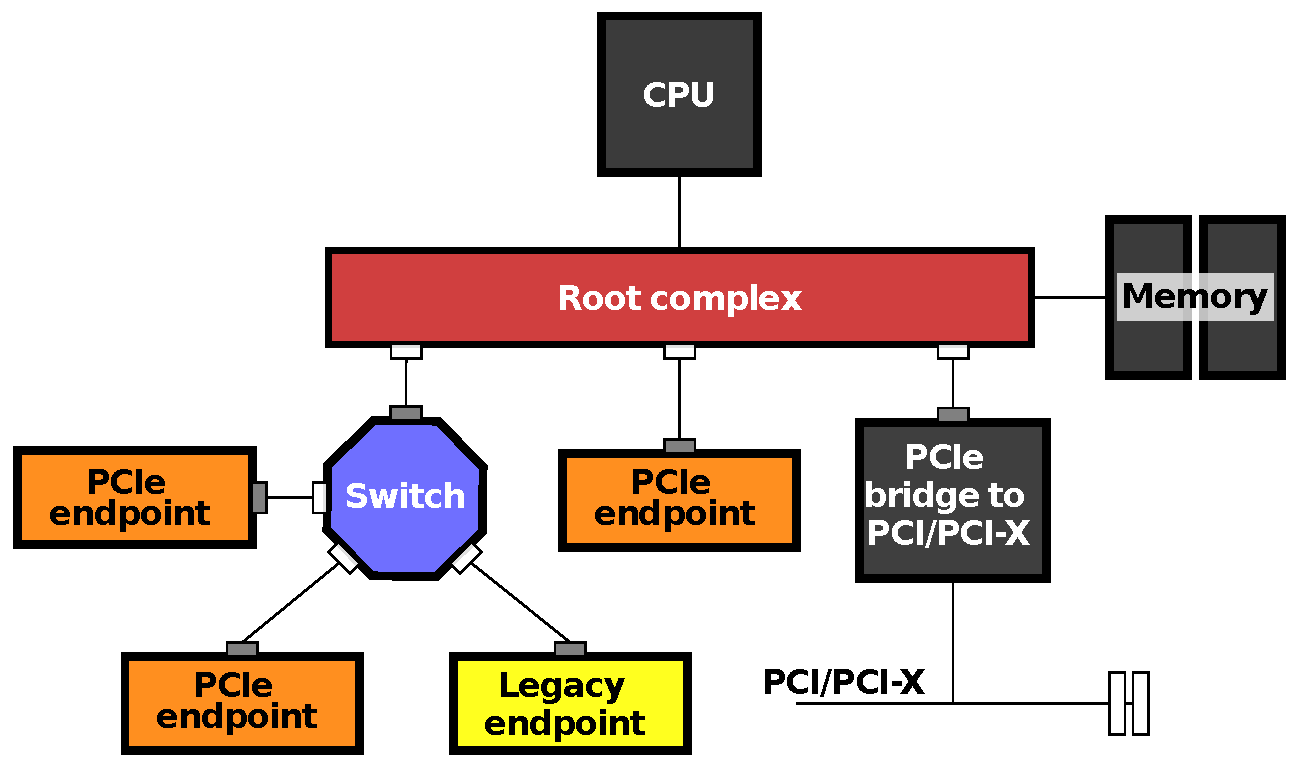
\includegraphics[height=0.5\textheight]{img/04.Example_PCI_Express_Topology.pdf}
    \end{figure}
    \begin{itemize}
        \item Северный мост трансформироавлся в \href{https://en.wikipedia.org/wiki/Root_complex}{Root Complex}, в современные процессоры обычно встраивается на кристалл, реже --- отдельным кристаллом в том же корпусе
        \item Южный мост «размазался»
        \item Некоторые традиционно «не периферийные» устройства, например ПЗУ (точнее ППЗУ) доступны через последовательную шину
    \end{itemize}
\end{frame}

\begin{frame}{PCI Express: Полосы, Совместимость разъёмов разной ширины}
	\begin{figure}
        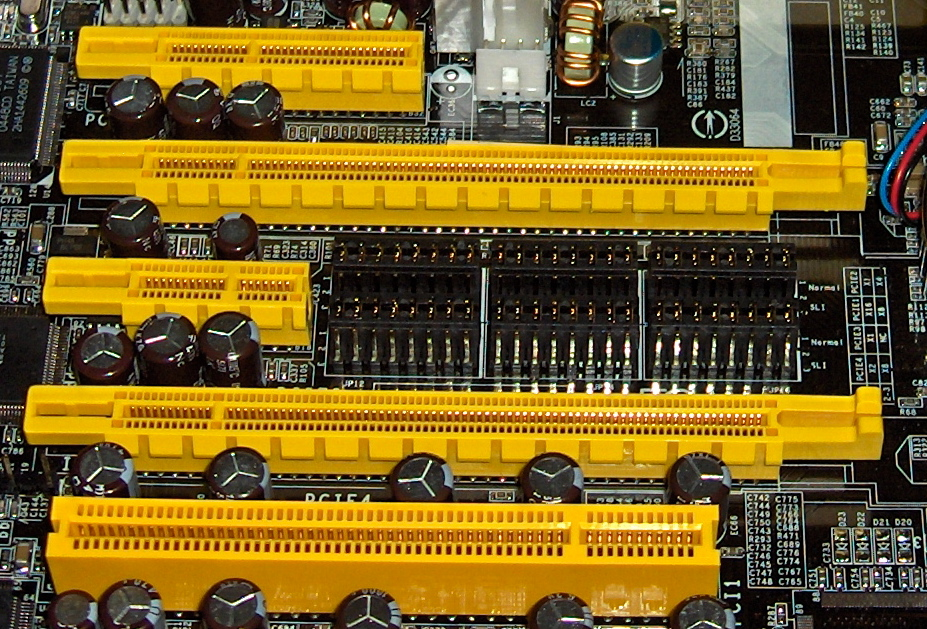
\includegraphics[height=0.5\textheight]{img/04.PCI-E_PCI_slots.jpg}
        \caption{\href{https://en.wikipedia.org/wiki/PCI_Express}{Разные разъёмы PCI-E (+ 1 PCI)}}
    \end{figure}
    \begin{itemize}
        \item Разные версии стандарта --- разные скорости
        \item Передача данных \emph{пакетами}, в зависимости от длины разъёма --- от 1 до 16 пакетов одновременно
        \begin{itemize}
            \item Устройства и разъёмы разной длины [обычно] совместимы друг с другом, если их можно соединить механически
            \begin{itemize}
                \item Короткое устройство будет работать в длинном разъёме
                \item Длинное устройство может иметь пропилы на контактной площадке, либо вставляться в «открытый» разъём
            \end{itemize}
        \end{itemize}
    \end{itemize}
\end{frame}

\begin{frame}{PCI Express: Скорости}
    \begin{figure}
        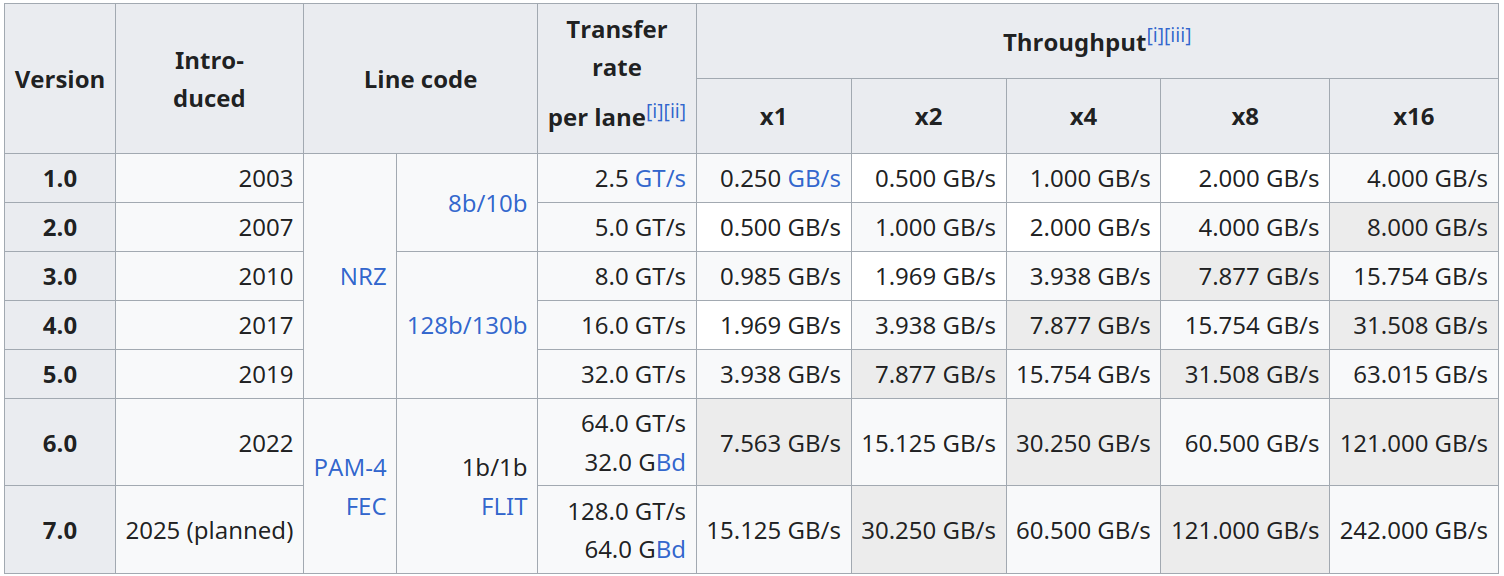
\includegraphics[height=0.5\textheight]{img/04.PCI-E_Speeds.png}
        \caption{Скорости PCI Express по данным \href{https://en.wikipedia.org/wiki/PCI\_Express\#History\_and\_revisions}{Википедии} и \href{https://web.archive.org/web/20131019114456/http://www.pcisig.com/news_room/faqs/pcie3.0\_faq/PCI-SIG\_PCIe\_3\_0\_FAQ\_Final\_07102012.pdf}{Peripheral Component Interconnect Special Interest Group}}
    \end{figure}
\end{frame}

\begin{frame}{Mini PCI Express, mSATA и M.2}
    \begin{figure}
        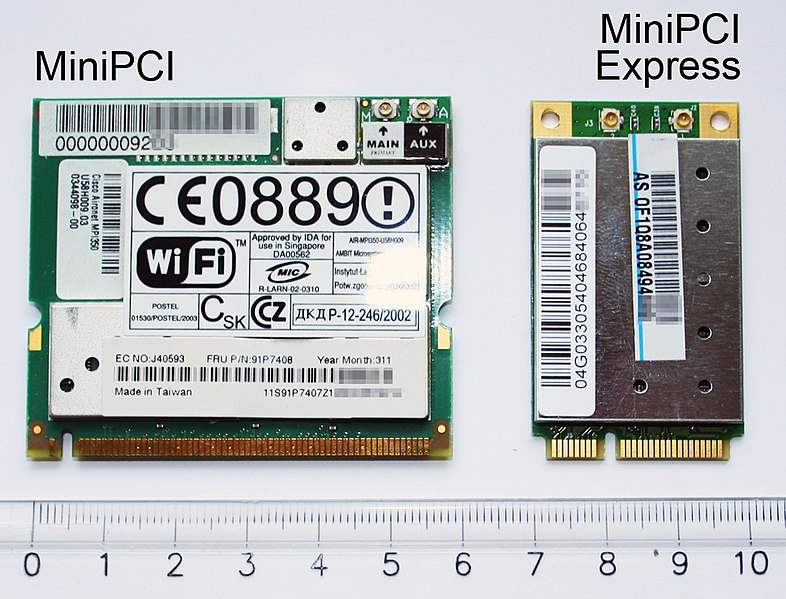
\includegraphics[height=0.35\textheight]{img/04.MiniPCI_and_MiniPCI_Express_cards.jpg}
        \caption{\href{https://en.wikipedia.org/wiki/PCI_Express\#MINI-CARD}{Mini PCI \& Mini PCI-E}}
    \end{figure}
    \begin{figure}
        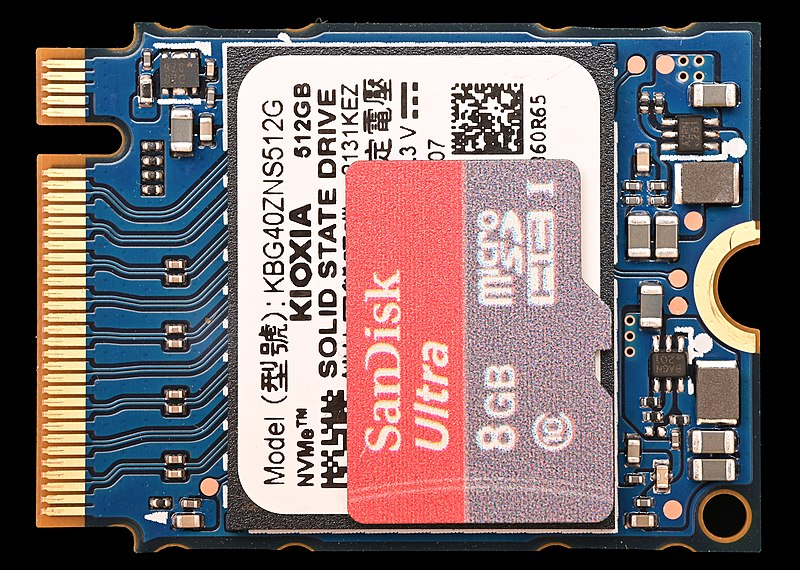
\includegraphics[height=0.25\textheight]{img/04.M.2_Carg.jpg}
        \caption{\href{https://en.wikipedia.org/wiki/M.2\#Form_factors_and_keying}{M.2}
        \href{https://en.wikipedia.org/wiki/M.2\#/media/File:SATA_Express_interface.svg}{использует одинаковый электический и сигнальный интерфейсы с mSATA},\\это типичная практика, и об этом ниже
        }
    \end{figure}
\end{frame}

\section{Интерфейсные шины USB и Thunderbolt}

\begin{frame}{История USB}

\begin{itemize}
    \item Используется с середины 1990-х
    \item Идеи:
    \begin{itemize}
        \item Универсальность
        \item Возможность под/отключения на ходу
        \item Механически прочный разъём c мощным питанием
        \item Изначально — не очень высокая скорость: у хорошо настроенного параллельного порта IEEE 1284 (LPT) скорость выше, чем у USB 1.X
    \end{itemize}
\end{itemize}
\pause
\href{https://en.wikipedia.org/wiki/USB\#Connector_type_quick_reference}{Разъёмы за более, чем 25-летнюю историю}

\end{frame}

\section*{}

\begin{frame}{Упражнения и вопросы}
	\begin{block}{Упражнения}
		\begin{itemize}
			\tightlist
			\item
			Попытайтесь идентифицировать все компьютерные разъёмы, которые вы можете встретить
		\end{itemize}
	\end{block}

	\begin{block}{Вопросы}
		\begin{itemize}
			\tightlist
            \item
            Что такое Root Complex?
            \item
            В чём смысл использования последовательных шин расширения?
            \item
            Приведите примеры протоколов, использующих одинаковые электрические и сигнальные интерфейсы
		\end{itemize}
	\end{block}
\end{frame}

\postamble
\end{document}
